\chapter{INTRODUÇÃO}\label{CAP:introducao}
%\thispagestyle{empty}

\section{CONTEXTO HISTÓRICO E RELEVÂNCIA DO TEMA}
No Brasil, o modal rodoviário é o que possui a maior representatividade entre os existentes e ainda hoje se encontra em constante expansão. No período de 2001 a 2015, as rodovias pavimentadas cresceram 23,2\% e em 2015 a extensão de rodovias pavimentadas no país chegou a 210,6 mil quilômetros. No mesmo período, a frota de veículos aumentou 184,2\%, segundo dados do Departamento Nacional de Infraestrutura de Transportes (DNIT). 

Apesar de este cenário indicar a necessidade de um crescente investimento no setor, o que se observa na realidade é que as verbas destinadas a ele estão estagnadas ou até mesmo em queda. Sem investimentos e com uma solicitação crescente, os pavimentos das rodovias brasileiras apresentam em geral uma qualidade bastante comprometida. A situação das rodovias federais é especialmente delicada, uma vez que grande parte da malha já superou a vida útil dos projetos originais. Segundo uma pesquisa realizada pela Confederação Nacional do Transporte \cite{cnt}, 48,3\% das rodovias avaliadas apresenta algum tipo de problema, tendo classificação regular, ruim ou péssima (Figura \ref{Fig:class}). 

\begin{figure}[!ht]
\centering
\caption{Classificação do estado dos pavimentos nas rodovias federais brasileiras}
{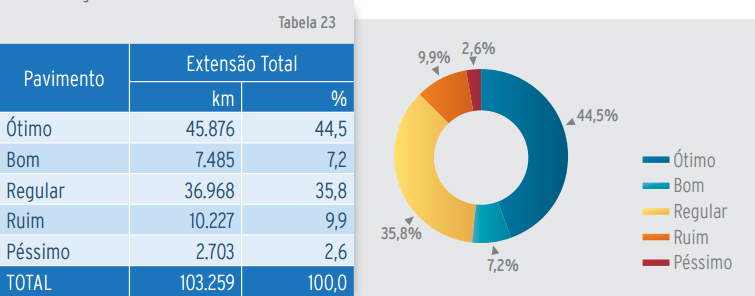
\includegraphics[scale=0.7]{figures/class.jpg}}\\
\makebox[\width]{Fonte: Confederação Nacional do Transporte (2016)} 
\label{Fig:class}
\end{figure}

Sabe-se que problemas de diversas naturezas decorrem da ausência de manutenção das rodovias e várias pesquisas já foram realizadas no sentido de quantificar esses prejuízos, como \citeonline{bartholomeu}, que estudou os impactos econômicos e ambientais do estado de conservação das rodovias. A \citeonline{cnt} estima que o custo operacional possa ser até 91,5\% mais alto nas vias em que o pavimento é considerado péssimo. O aumento do custo é referente a gastos com a manutenção dos veículos, de lubrificantes, de pneus e de freios além do aumento no consumo de combustível. 
Outro aspecto afetado é o ambiental, visto que a emissão de gases poluentes como o $CO_2$ está diretamente ligada ao consumo de combustíveis fósseis. Além disso, vias com características impróprias de textura também podem gerar um aumento significativo no desgaste de pneus, uma questão importante a ser considerada, uma vez que a borracha da qual eles são fabricados não é biodegradável.

Há ainda o comprometimento de outros aspectos, como o conforto e a segurança dos usuários. De acordo com a \emph{World Road Association} \cite{celko} uma redução do coeficiente de atrito abaixo de 0,45 ocasiona até 20 vezes mais acidentes, quando este atinge um índice menor que 0,30 o risco aumenta cerca de 300 vezes.

Em um cenário mais amplo podemos relacionar também a condição das rodovias ao preço final dos produtos comercializados. No Brasil, o transporte de cargas é realizado em sua grande maioria por meio de rodovias, desta forma, todos os aumentos dos custos operacionais citados anteriormente são embutidos no preço final dos produtos que utilizam este modal. Isso implica na perda de competitividade dos produtos brasileiros no mercado internacional, afetando a economia do país. 

Tendo em vista os fatores referidos acima, podemos compreender a importância de se tratar com seriedade a questão de avaliação e reparo das rodovias do país. Ao identificar esta necessidade crescente, constatou-se a insuficiência dos métodos existentes até o presente momento, os quais são bastante limitados, seja por sua complexidade, alto custo dos equipamentos ou pela imprecisão dos ensaios. Acredita-se, portanto, ser de fundamental importância o desenvolvimento de métodos rápidos e econômicos para que se possa avaliar a condição dos pavimentos de forma eficiente, sem inferir em altos custos.

Neste cenário, propõe-se um método alternativo para a avaliação da rugosidade de pavimentos através de equipamentos de escaneamento tridimensional a laser, os quais vêm se tornando cada vez mais acessíveis e podem ser encontrados inclusive, em diversas universidades brasileiras.

\section{OBJETIVOS}
O presente trabalho tem como principais objetivos: 

\begin{itemize}

\item Demonstrar a aplicação da técnica de escaneamento tridimensional a laser para classificação da textura de pavimentos;

\item Comparar os resultados computacionais com os dados obtidos experimentalmente e verificar a precisão do método; 

\item Esclarecer as vantagens e insuficiências do método e abrir espaço para que outras propostas possam surgir, propiciando a difusão dos meios de controle da qualidade dos pavimentos no país. 
\end{itemize}

\section{ORGANIZAÇÃO DO TRABALHO}

O Capítulo \ref{CAP2} traz uma revisão de literatura, abordando a definição de alguns conceitos essenciais para viabilizar o entendimento do método e a descrição de estudos anteriores pertinentes ao tema.

O Capítulo  \ref{CAP3} apresenta os materiais e métodos utilizados neste trabalho, são descritas as especificações técnicas dos equipamentos utilizados, além da descrição dos ensaios realizados; 

O Capítulo  \ref{CAP4} apresenta os resultados dos métodos experimental e computacional e realiza uma comparação entre eles. São calculadas as variações entre os resultados como forma de verificar sua precisão; 

O Capítulo \ref{CAP5} traz as conclusões inferidas a partir dos resultados obtidos e analisa possibilidades de expansão deste tema em futuros trabalhos.


